\subsection{\acrshort{orb}}\label{sec:orb_stats}
\begin{figure}[H]
\begin{subfigure}[t]{0.45\linewidth}
    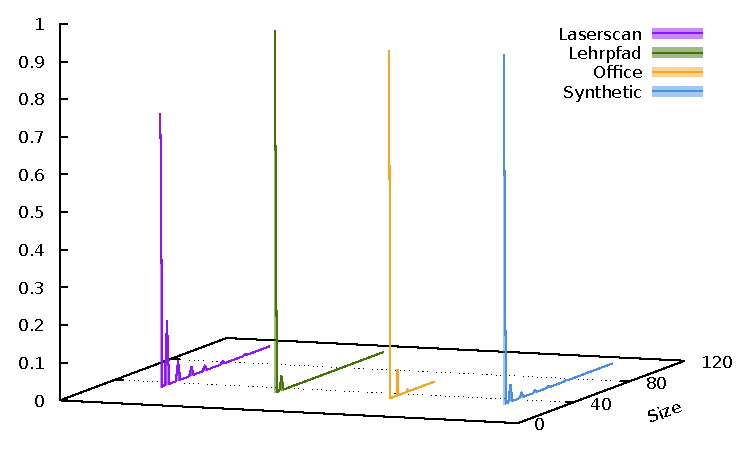
\includegraphics[width=\linewidth]{chapter06/results/ORB/flexion/size.pdf}%
    \caption{Flexion Image Keypoint Sizes}
\end{subfigure}\quad
\begin{subfigure}[t]{0.45\linewidth}
    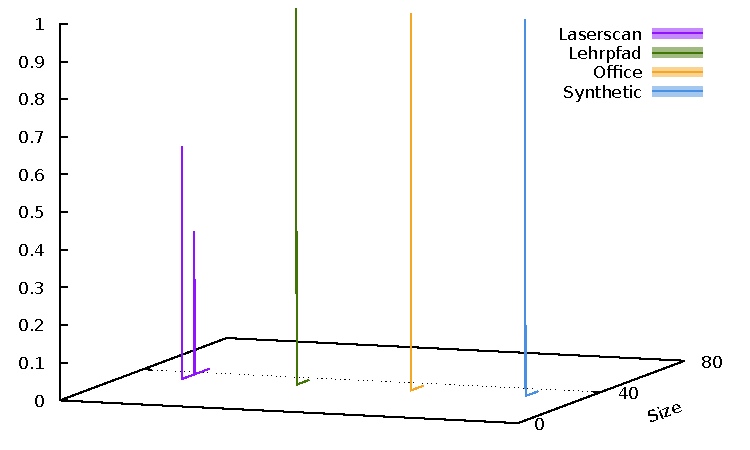
\includegraphics[width=\linewidth]{chapter06/results/ORB/bearing/size.pdf}
    \caption{Bearing-Angle Keypoint Sizes}
\end{subfigure}
    \caption{Comparing Keypoint Sizes}
\end{figure}
\begin{figure}[H]
\begin{subfigure}[t]{0.45\linewidth}
    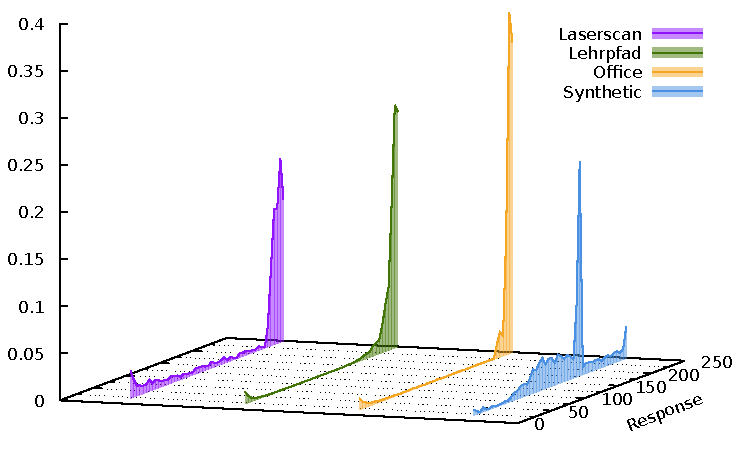
\includegraphics[width=\linewidth]{chapter06/results/ORB/flexion/response.pdf}%
    \caption{Flexion Image Keypoint Responses}
\end{subfigure}\quad
\begin{subfigure}[t]{0.45\linewidth}
    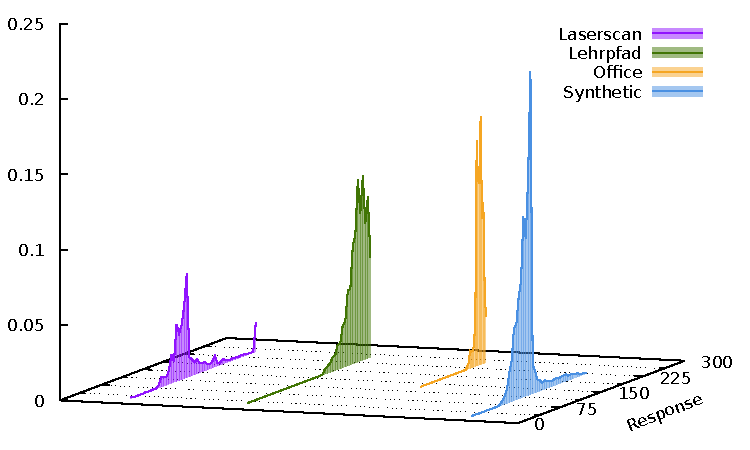
\includegraphics[width=\linewidth]{chapter06/results/ORB/bearing/response.pdf}
    \caption{Bearing-Angle Keypoint Responses}
\end{subfigure}
    \caption{Comparing Keypoint Responses}
\end{figure}
\begin{figure}[H]
    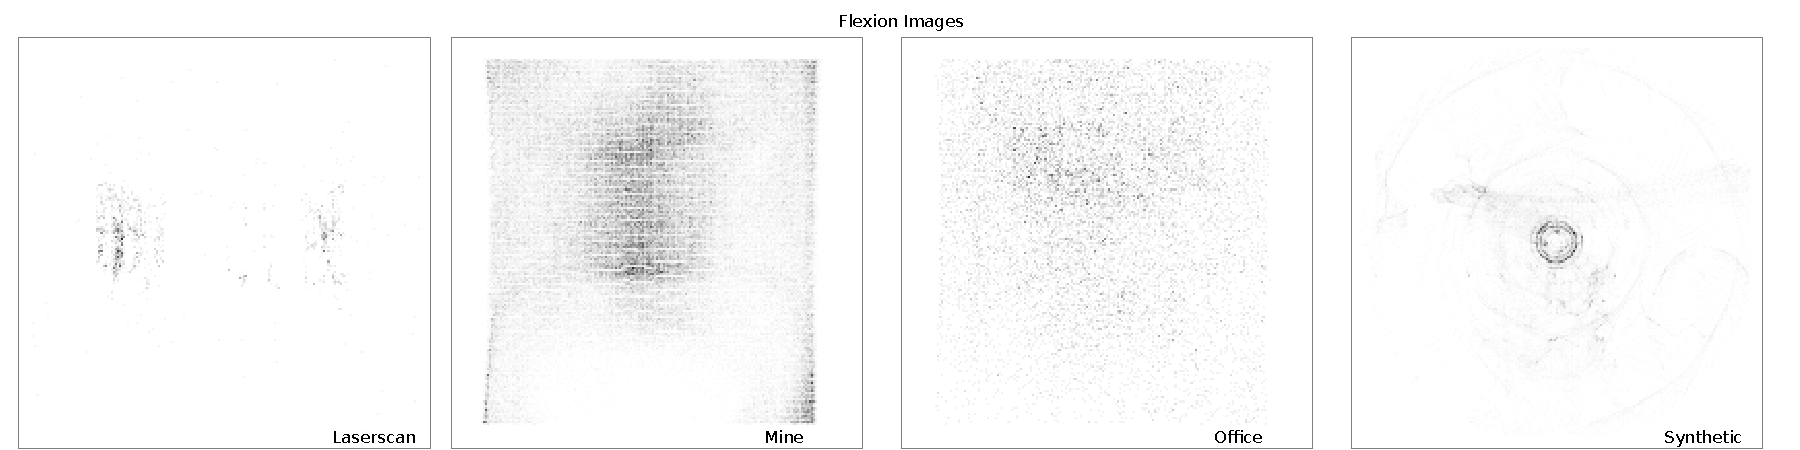
\includegraphics[width=\linewidth]{chapter06/results/ORB/flexion/distribution.pdf}\\
    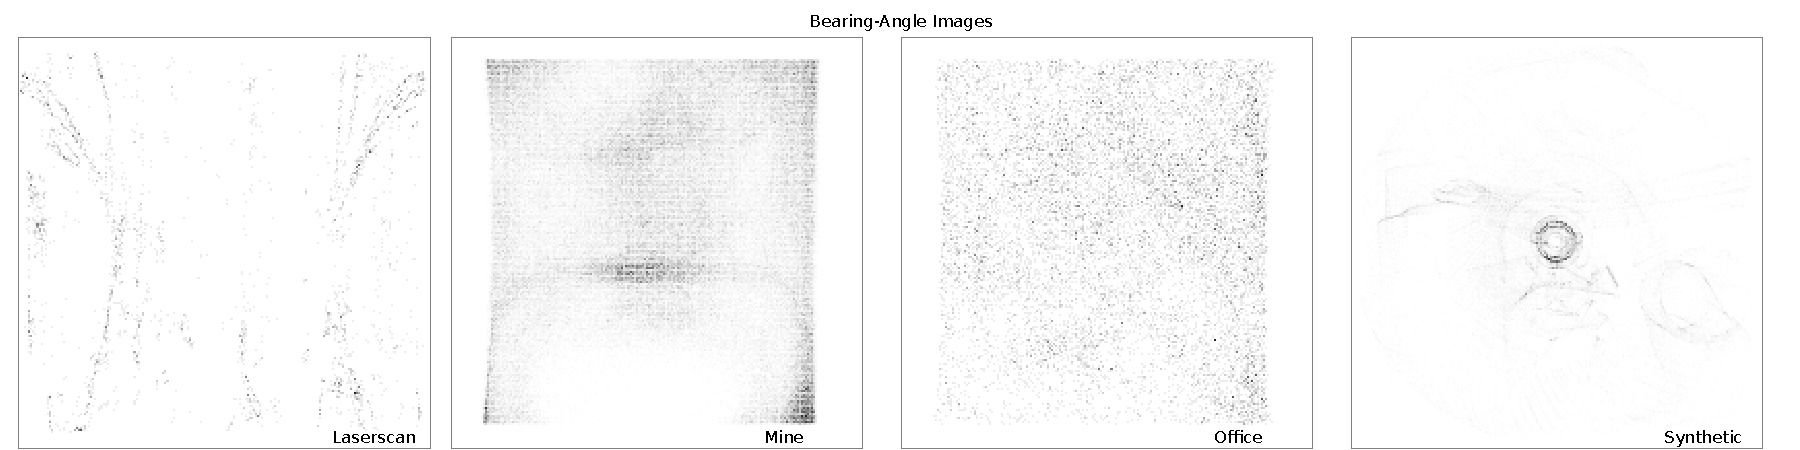
\includegraphics[width=\linewidth]{chapter06/results/ORB/bearing/distribution.pdf}%
    \caption{Keypoint Distribution for Flexion and Bearing.}
\end{figure}
